\begin{center}
\Huge
Sidste aflevering 1.g
\end{center}
\section*{Opgave 1 (uden hjælpemidler)}
Forkort udtrykket
\begin{align*}
\frac{a^2-b^2}{a-b} -b.
\end{align*}

\section*{Opgave 2 (uden hjælpemidler)}
Bestem følgende sum:
\begin{align*}
\frac{6+7}{12} + \frac{9-1}{6}.
\end{align*}

\section*{Opgave 3 (uden hjælpemidler)}
\stepcounter{section}
Løs ligningen 
\begin{align*}
2x+6=20.
\end{align*}

\section*{Opgave 4 (uden hjælpemidler)}
Et polynomium $f$ er givet ved
\begin{align*}
f(x) = 2x^2+2x-12.
\end{align*} 
\begin{enumerate}[label=\roman*)]
\item Bestem koefficienterne for $f$.
\item Afgør, hvor $f$ skærer $x$-aksen.
\end{enumerate}

\section*{Opgave 5 (uden hjælpemidler)}
På Fig. \ref{fig:polys} ses parablerne $P_1$, $P_2$ og $P_3$ for andengradspolynomierne $f$, $g$ og $h$ givet ved henholdsvist
\[
	f(x) = x^2-4,
\]
\[
	g(x) = -2x^2+3x+3,
\]
og
\[
	h(x)= x^2-3x-4.
\]
\begin{figure}[H]
\centering
	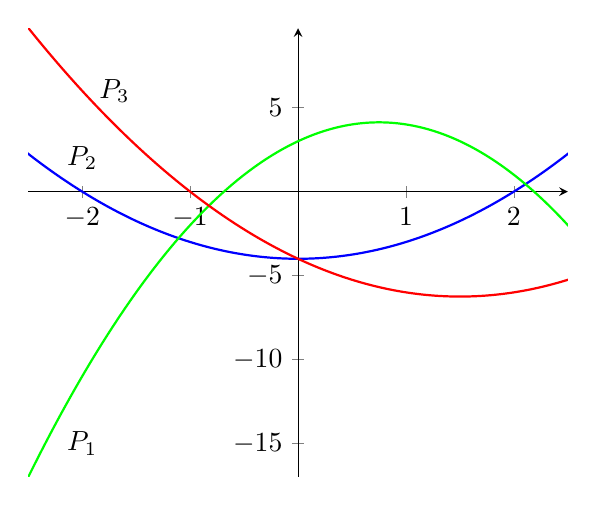
\begin{tikzpicture}
	\begin{axis}[axis lines = middle,
	xmin = -2.5, xmax = 2.5]
	\addplot[samples = 1000, color = blue, thick] {x^2-4};
	\addplot[samples = 1000, color = green, thick] {-2*x^2+3*x+3};
	\addplot[samples = 1000, color = red, thick] {x^2-3*x-4};
	\node at (axis cs: -2,-15) {$P_1$};
	\node at (axis cs: -2,2) {$P_2$};
	\node at (axis cs: -1.7,6) {$P_3$};
	\end{axis}
	\end{tikzpicture}
	\caption{Parablerne $P_1$, $P_2$ og $P_3$}
	\label{fig:polys}
\end{figure}
\begin{enumerate}[label=\roman*)]
\item Afgør, hvilken af funktionerne $f$, $g$ og $h$ der passer til hver af parablerne $P_1$, $P_2$ og $P_3$.
\end{enumerate}

\section*{Opgave 6 (uden hjælpemidler)}
En potensfunktion $f$ givet ved
\begin{align*}
f(x) = b\cdot x^a
\end{align*} skærer gennem punkterne $(1,10)$ og $(10,1000)$.
\begin{enumerate}[label=\roman*)]
\item Brug topunktsformlen for potensfunktioner til at bestemme $a$ og $b$.
\item Bestem $f(3)$.
\end{enumerate}

\section*{Opgave 7 (uden hjælpemidler)}
To linjer er givet ved ligningerne
\begin{align*}
2x+4y = 0
\end{align*}
og 
\begin{align*}
x+y = 2.
\end{align*}
\begin{enumerate}[label=\roman*)]
\item Find skæringspunktet $P$ mellem de to linjer.
\end{enumerate}

\section*{Opgave 8 (uden hjælpemidler)}
To vektorer $\vv{u}$ og $\vv{v}$ er givet ved
\begin{align*}
\vv{u}= \begin{pmatrix}
 3 \\ x
\end{pmatrix} 
\end{align*}
og 
\begin{align*}
\vv{v}= \begin{pmatrix}
 -1 \\ 1
\end{pmatrix} 
\end{align*}
\begin{enumerate}[label=\roman*)]
\item Bestem længden af $\vv{u}$, når $x = 4$.
\item Bestem $x$, så de to vektorer er parallelle. 
\end{enumerate}
\section*{Opgave 9 (med hjælpemidler)}
Et taxafirma TaxA skal have 11kr per kørt km, og det koster 40kr at begynde en rejse hos TaxA. Et konkurrerende firma TaxB tager 12.5 kr per kørt km, men det er til gengæld gratis at begynde en rejse med dette firma. 
\begin{enumerate}[label=\roman*)]
\item Indfør passende variable og bestem en model for prisen for at køre med begge taxafirmaer som funktion af antallet af kørte km. 
\item Tegn prisen som funktion af den kørte afstand i et koordinatsystem. 
\item Bestem, hvornår langt du skal køre, før TaxA er det billigste firma. 
\end{enumerate}

\section*{Opgave 10 (med hjælpemidler)}
En appelsinbonde ønsker at bestemme sammenhængen mellem radius på hans appelsiner og mængden af juice, han får per appelsin. Han prøver derfor at presse appelsiner med forskellig radius, og måler mængden af juice per appelsin. Hans opsamlede data kan ses af Tab. \ref{tab:juice}.
\begin{table}[H]
\begin{tabular}{c|c|c|c|c|c|c|c|c|c|c}
Radius (cm) & 2 & 2.1 & 2.15 & 2.3 & 2.4 & 2.6 & 2.9 & 3.05 & 3.4 & 3.5\\ \hline
Juice (dL) & 0.2 & 0.22 & 0.19 &0.24 & 0.31 & 0.45 & 0.55 & 0.59 & 0.85 & 0.97
\end{tabular}
\caption{Juice fra appelsiner}
\label{tab:juice}
\end{table}

\begin{enumerate}[label=\roman*)]
\item Bestem den lineære funktion samt den potensfunktion, der bedst beskriver mængden af juice som funktion af radius af appelsinerne. 
\item Plot residualerne for de to modeller og afgør, hvilken model der beskriver sammenhængen bedst.
\end{enumerate}
En unavngiven virksomhed påstår, at der til 1.75L af deres juice skal bruges 16 søde appelsiner. 

\begin{enumerate}[label=\roman*)]
\setcounter{enumi}{2}
\item Hvor store skal disse appelsiner i følge din model være, hvis virksomhedens påstand skal være korrekt (og appelsinerne er lige store)?
\end{enumerate}

\section*{Opgave 11 (med hjælpemidler)}
En eksponentialfunktion $f$ givet ved 
\begin{align*}
f(x) = b\cdot x^a
\end{align*}
har halveringskonstant $T_{1/2} = 3$. Desuden går funktionen gennem punktet $(1,2)$. 
\begin{enumerate}[label=\roman*)]
\item Bestem $a$
\item Bestem $b$. 
\item Løs ligningen $f(x) = 1$. 
\end{enumerate}